\section{Results}
	Painting segmentation: 88.57 \% correct segmentation
	\todo{qualitative as well as quantitative}
	
	\todo{quantitative: graphs, tables, roc-curves, f1-scores, ...}
	
	\todo{qualititative: technisch, show where and why the method succeeds or fails, pictures of easy and difficulty cases}
	
	Because our method relies heavily on edge detection, there are cases where this could have a negative impact. In many cases, there is a shadow underneath the painting, as shown on figure \ref{fig:negative_case_shadow}.
	
	\begin{figure}
		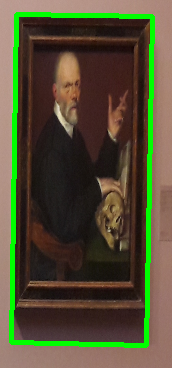
\includegraphics[width=\linewidth]{negative_case_shadow}
		\caption{An example of a shadow underneath the painting. This usually results in the segmentation algortihm to include this shadow as part of the painting because of the strong edge.}
		\label{fig:negative_case_shadow}
	\end{figure}

	\todo{stukje hierboven ook kwalitatief?}

\subsection{Qualitative analysis}
In this subsection, we will present a qualitative analysis of our algorithm. We will discuss its strengths, flaws and, with each point, present an example case to help as a visual aid. The flaws in particular help paint a picture of what can be done better in a future iteration of the algorithm. 


One of the algorithm's major strengths lies in its simplicity. The block diagram shows a very linear approach to the problem with concrete begin- and endpoints. Though machine learning is often used in the field of computer vision and has a lot of benefits, the algorithm does not employ it. We do not deny its usefulness and believe that it may be beneficial to implement it in a future version of the algorithm \todo{waar nodig?, kan zijn dat ML gebruikt wordt bij matching}. Even though the algorithm's simplicity is presented as one of its strengths, it can also be considered as one of its weaknesses, much like a double edged sword.


Furthermore, the algorithm works relatively fast for matching and determining the location of a potential user using a single image. Table \todo{tbl} gives an overview of the average elapsed time when running the algorithm on a single image. 
\todo{chart met timing van algoritme voor 1 afbeelding}


In addition, the use of ORB causes the results of each program run to be invariant given the same input image, implying a deterministic nature. This is of course on the premise that certain parameters such as the Canny thresholds remain the same between runs. Figures \todo{fig} and \todo{fig} shows how two images have the same match and detected keypoints between two runs. However, due to not detecting different potential candidate matches between runs results in the algorithm never being able to present a different solution for the given image.


On top of that, the algorithm is resilient when it can not successfully segment an image. The default behaviour is trying to find a frame, extract it, and using it as the input of the matching stage of the algorithm. If no frame can be found, rather than ignoring the current video frame or image, we supply the entire thing to be matched. This may slow the matching stage down by a small margin but has the benefit of still being able to spit out a potential positive match. Figure \todo{fig} shows an example where an entire frame is supplied to the matching function, but still manages to find a correct match.


As was hinted in the previous point, supplying a full frame or image to the matching phase may slow things down. The input image's size definitely affects the time needed to complete in a negative way. Therefore, images used for the segmentation and matching phases are resized to between \verb|25%-50%| their original size. This may result in some loss of precision but should not affect the overall efficiency of the algorithm. Table \todo{tbl} shows that resizing an image from the query set to a quarter of its size quadratically decreases the amount of pixels needed to evaluate. The same resizing is applied to the building stage of the database.


Another problem arises due to an assumption in the matching stage. A match is determined by the smallest sum of distances calculated over the matches between two images. This assumption works well when the amount of matches is fixed between every match between the query image and the training set. ORB detects keypoints and associates descriptors up to a maximum of 200. But what if it can not detect a lot of keypoints, maybe even none? Figure \todo{fig} shows how paintings that have a relative 'flat' surface without discerning features (even to the naked eye) have trouble being matched to a picture in the data set. Suppose that the segmentation phase detects such a painting and supplies it to the matching phase. A cascade of erroneous matches and room localizations may occur. The inverse is also true, as having an entry in the data set with few keypoints can result in a painting with many keypoints being wrongfully matched with a 'flat' one.


The final major flaw that will be presented lies in the matching phase: matching a painting is done by doing a linear lookup in the database. For a single image this does not pose that much of a problem. The same can not be said when we expanded our algorithm to analyze the frames of a video. This slowdown is mitigated through two changes to the original algorithm. First, we run it only every 30 or so video frames which is equivalent to around 1 second in real life. Suppose the user is using their smart phone's camera, even when running, it will take some time to cross from one room to the other. Finally, the algorithm offloads the matching procedure to a multithreading environment, freeing the video code from freezing. But what causes this freezing in the first place? 


Considering there are 688 pictures in the database, coupled with the keypoints and descriptors that were extracted during the prebuilding phase, are matched with the descriptors of the segmented painting results in a total.

Furthermore, there is also no stop condition to the lookup.
This suggests that our matching code has $O(n^{2})$ behaviour.
which with a small amount of pictures is not a factor that we can simply leave. A possible solution to this problem may lie in other journals \todo{ref naar boek/conference over bag of words/large databases}. \todo{laatste paragraaf herschrijven} \todo{https://github.com/opencv/opencv/blob/master/doc/py_tutorials/py_feature2d/py_matcher/py_matcher.markdown}